%% ------------------------------------------------------------------------- %%
\chapter{Test-Driven Development}
\label{cap:tdd}

Test-Driven Development (TDD) é a arte de produzir testes automatizados para código de produção, usando
esse processo para guiar o design e a programação. Para cada pequeno pedaço de funcionalidade, o desenvolvedor
deve primeiro escrever um teste que especifique e valide o que o código irá fazer. O programador então produz
somente o código necessário para fazer esse teste passar. Então ele refatora (simplifica e clareia) tanto o
código de produção quanto o código de testes \cite{agilealliance-tdd} \cite{tdd-taxonomy}.

TDD é uma importante prática na Programação Extrema (XP) \cite{XPExplained} já que, como sugerido pelas práticas
ágeis, o design de um software deve emergir conforme o software cresce. E, para responder rapidamente a essas
alterações, é necessário um constante \textit{feedback} sobre a qualidade interna e externa do código, e TDD
provê isso já que faz com que o teste de unidade seja o primeiro cliente real da classe que o programador ainda
vai implementar, e isso faz com que ele pense melhor a respeito do comportamento que ele espera dessa classe. Além disso,
a suíte de testes gerada dá segurança ao programador no momento de uma refatoração pois, caso ele cometa um erro,
algum dos testes provavelmente irá falhar, avisando-o imediatamente sobre o problema.

TDD faz com que esse simples processo de escrever um teste antes de escrever o código
sirva para ajudar o time a entender as funcionalidades que os usuários do sistema precisam e 
a entregar essas funcionalidades de maneira confiável e previsível \cite{GOOS}. TDD usa os testes para clarificar as expectativas
sobre o que um pedaço de código deve fazer [TODO 3]. Além disso, ele cria uma medida concreta de falha, que são os testes de 
unidade que estão falhando. Com essa medida em mãos, o objetivo do programador naquele momento é simplesmente fazer o teste passar. É um
objetivo claro e bem definido, e permite ao programador focar naquele pequeno pedaço de funcionalidade e no trecho de código que ele 
deve escrever para fazer o teste passar. Ron Jeffries resume o objetivo de TDD a "código claro que funciona" \cite{TDDByExample}. 

Na prática, TDD obriga que o programador escreva
um código novo apenas se houver um teste automatizado falhando, e faz com que ele remova duplicação de dados e de código constantemente. 
Essas duas regras implicam no seguinte ciclo: o programador primeiro deve escrever um pequeno teste que falhe (ou que até mesmo não compile), 
em seguida deve fazer o teste passar de maneira mais rápida possível e, por fim, deve refatorar toda a duplicação criada \cite{TDDByExample}. 
Esse ciclo, exemplificado na figura \ref{fig:red-green-refactor} é também conhecido como 
Vermelho-Verde-Refatora (ou Red-Green-Refactor), já que lembram as cores que o programador geralmente 
vê quando faz TDD: o vermelho geralmente significa que o teste está falhando e o verde quando o teste foi executado com sucesso.

\begin{figure}
  \centering
  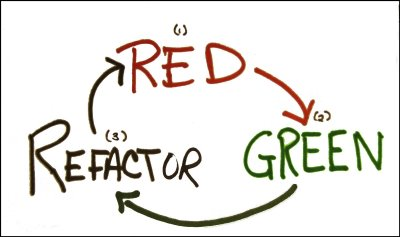
\includegraphics[scale=0.6]{ciclo-tdd}
  \caption{O ciclo Vermelho-Verde-Refatora}
  \label{fig:red-green-refactor}
\end{figure}

TDD apareceu para o mundo de desenvolvimento de softwares em 2001, quando Kent Beck publicou seu trabalho sobre Programação Extrema \cite{XPExplained},
onde TDD era uma das práticas citadas por ele como essenciais para o processo de desenvolvimento. Conhecida também
por \textit{Test-First Programming} (Programação Testando Primeiro), \textit{Test-Driven Design} (Design Guiado pelos Testes) ou 
\textit{Test-First Design} (Design Testando Primeiro), sua popularidade cresceu junto com o aumento de popularidade da própria Programação Extrema. 
Mas, nos últimos tempos, TDD tem recebido uma grande atenção entre os pesquisadores e profissionais da indústria, mesmo em equipes não-ágeis, já que
é dito que a sua prática aumenta tanto a qualidade interna do código, aumentando sua coesão, diminuindo seu acoplamento e tornando
o código mais simples, quanto a qualidade externa, diminuindo o número de defeitos.

\section{O Ciclo de TDD} 
\label{sec:tdd-ciclo}

De forma mais ampla, podemos definir o ciclo de TDD da seguinte maneira \cite{TDDByExample}:

\begin{enumerate}
	\item adicione um teste; 
	\item rode todos os testes e veja o novo teste falhar; 
	\item escreva o código mais simples que faça o teste passar; 
	\item rode todos os testes e veja o novo teste passar; 
	\item refatore para remover duplicação de dados e de código.
\end{enumerate}

A figura \ref{fig:tdd} mostra a ordem que as atividades são feitas. 
As sub-seções abaixo visam explicar cada passo do ciclo de forma mais detalhada, explicando a motivação e o esperado 
em cada um deles.

\begin{figure}
  \centering
  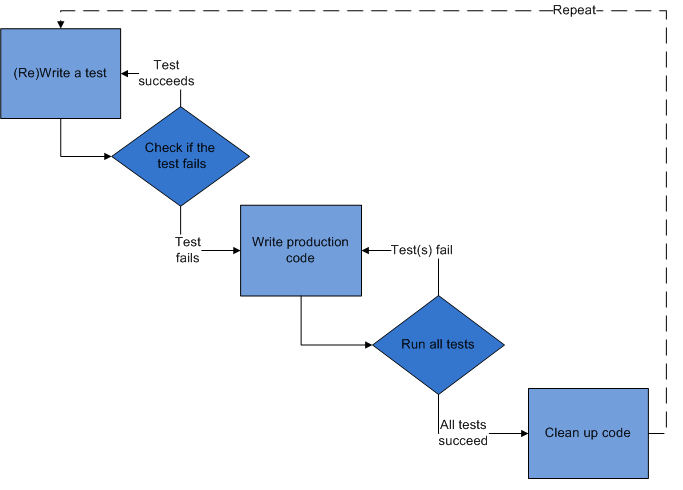
\includegraphics[scale=0.6]{tdd}
  \caption{O Ciclo de Test-Driven Development (retirado da Wikipedia \cite{figura-tdd-wiki}) }
  \label{fig:tdd}
\end{figure}

\subsection{Adicionar um teste}

O primeiro passo do ciclo é escrever um teste para uma nova funcionalidade. Para isso, o programador deve primeiro entender a funcionalidade 
que ele deseja implementar, e dessa forma entender melhor o requisito antes de escrever qualquer linha de código.
Esse teste falhará, afinal a funcionalidade ainda não foi implementada. 

Esse é um passo muito importante do processo, já que o teste que o programador vai escrever é o primeiro cliente da classe que está
prestes a implementar. Nesse momento o programador decide não somente sobre a interface que essa classe terá (como nomes dos métodos,
parâmetros, tipos de retorno e exceções a serem lançadas) como também sobre o comportamento que ele espera dessa classe (como 
os resultados de acordo com as diferentes entradas) \cite{GOOS}.

\subsection{Rodar todos os testes e ver o novo teste falhar}

Nesse momento o programador roda todos os seus testes de unidade e verifica se o teste escrito no passo anterior realmente falhou. Em um
primeiro momento esse passo pode parecer desnecessário, pois o programador escreveu um teste para uma funcionalidade que ele ainda nem
implementou, e portanto o teste irá falhar. 

Mas, na prática, esse teste pode não falhar, indicando alguns possíveis problemas, como: talvez o código da classe que está sendo testada
não está reagindo da maneira que o programador pensou que estava (afinal ele esperava por um determinado comportamento quando na verdade a
classe apresentou outro); problemas na implementação do teste, afinal teste também é código, e assim como o código de produção, ele é
totalmente suscetível a falhas.
Portanto, pode-se concluir que ver o novo teste falhar ajuda o programar a validar tanto o código de teste quanto o seu conhecimento
sobre a classe que está sendo testada. 

\subsection{Escreva o código mais simples que faça o teste passar}

O programador deve então escrever o código mais simples possível que faça o teste passar. Nesse momento o programador não deve estar
focado em escrever a solução mais clara (pois isso será feito em um passo posterior), e sim realmente a mais simples.

O objetivo desse passo é evitar que o programador, ao invés de resolver o problema de maneira simples, por algum motivo
implemente uma solução mais complexa, e com isso acrescentando complexidade desnecessária no código. Algumas técnicas como
\textit{Implementação Óbvia} e \textit{Triangularização} \cite{TDDByExample}, discutidas com mais detalhes na seção \ref{sec:tdd-patterns}, 
podem ajudar o programador na tarefa de escrever a implementação mais simples possível.

Muitas vezes esse passo é mal entendido pelos programadores, que acabam por confundir o "mais simples" pelo o "mais simplório". 
A ideia de passos de bebê \cite{TDDByExample} é melhor detalhada na seção \ref{sec:tdd-baby-steps}.

\subsection{Rode todos os testes e veja o novo teste passar}

Assim que o programador escrever o código mais simples que faça o teste passar, ele deve rodar a suíte de testes novamente
para verificar que a nova implementação realmente faz o teste passar. Nesse ponto é importante que o programador rode a suíte 
completa de testes, pois a implementação pode ter feito o novo teste passar, mas pode ter quebrado testes antigos que já existiam na suíte. 
Caso algum teste antigo quebre, o programador deve então voltar um passo atrás, e tentar novamente escrever o código mais simples
que faça o teste que está quebrado passar.

Esse passo traz segurança ao programador durante todo o ciclo de desenvolvimento, pois rodando a suíte de testes inteira, 
ele rapidamente descobre se introduziu um erro em alguma outra parte do sistema. Essa é uma técnica conhecida na área de testes e é
chamada de \textit{testes de regressão} \cite{art-of-sw-testing}. Em TDD, e execução constante desses testes de regressão 
trazem outra vantagem que é a detecção do erro acontece basicamente no momento em que esse erro é introduzido, facilitando assim
o processo de correção do mesmo. Alguns estudos inclusive mostram que o programador ao fazer TDD passa menos tempo depurando o código
do que programadores que utilizam a abordagem tradicional (TODO janzen 5, george williams 9 artigo aniche).

\subsection{Refatore para remover duplicação de dados e de código}

No último passo do ciclo o programador agora deve refatorar o código escrito, procurando remover as duplicações de código ou de dados. 
Conforme comentado acima, o código escrito anteriormente era o mais simples, mas não necessariamente o mais claro possível. O programador
nesse momento tem total liberdade para refatorar, já que tem uma suíte de testes para garantir que o comportamento não será alterado.
Esse é um dos principais passos no ciclo, já que é aqui que o programador se preocupa em melhorar o seu código, tornando-o
mais claro e, por consequência, facilitando sua evolução.

Como TDD faz com que a prática de testes seja utilizada para receber informações sobre o design, 
a prática de refatoração é parte vital do processo já que o programador muda de ideia muitas vezes sobre a interface que determinada
classe deve ter, e para isso, faz uso de práticas de refatoração, já muito discutida na literatura \cite{fowler-refactoring} \cite{joshua-refactoring}.

\section{Um pequeno exemplo}
\label{sec:tdd-exemplo}

Suponha o desenvolvimento de uma classe responsável por calcular a sequência de Fibonacci. A primeira e mais simples funcionalidade que
vem a cabeça é retornar o primeiro elemento da sequência. O primeiro teste então é:

\begin{lstlisting}[frame=trbl]
@Test
public void deveRetornar0ParaOElementoZeroDaSequencia() {
	SequenciaDeFibonacci sequencia = new SequenciaDeFibonacci();
	assertEquals(0, sequencia.pegaValor(0));
}
\end{lstlisting}

Repare que esse trecho de código apresenta erros de compilação: a classe \textit{SequenciaDeFibonacci} ainda não existe. O primeiro
passo é resolver os erros de compilação, adicionando o seguinte código:

\begin{lstlisting}[frame=trbl]
public class SequenciaDeFibonacci {
	public int pegaValor(int sequencia) {
		return -1;
	}
}
\end{lstlisting}

Ao executar o teste, o JUnit retorna a seguinte mensagem: \textit{java.lang.AssertionError: expected:<0> but was:<-1>}, que significa que
o teste esperava que o método retornasse o valor 0, mas ao invés disso, retornou o valor -1. Com o teste falhando, o próximo passo é escrever
o código mais simples que faça o teste passar: nesse caso, basta fazer a função retornar 0.

\begin{lstlisting}[frame=trbl]
public class SequenciaDeFibonacci {
	public int pegaValor(int sequencia) {
		return 0;
	}
}
\end{lstlisting}

O próximo teste é fazer com que o método retorne 1 caso seja o primeiro elemento da lista. O programador então deve escrever o
seguinte teste:

\begin{lstlisting}[frame=trbl]
@Test
public void deveRetornar1ParaOPrimeiroElementoDaSequencia() {
	SequenciaDeFibonacci sequencia = new SequenciaDeFibonacci();
	assertEquals(1, sequencia.pegaValor(1));		
}
\end{lstlisting}

O teste falha. O programador agora deve fazer o teste passar, escrevendo o código mais simples possível:

\begin{lstlisting}[frame=trbl]
public int pegaValor(int sequencia) {
	return sequencia;
}
\end{lstlisting}

Para finalizar, a próxima funcionalidade é fazer com que o método, dado uma entrada maior que 1, retorne sempre a soma dos dois anteriores.
Para isso, o programador deve escrever um teste:

\begin{lstlisting}[frame=trbl]
@Test
public void deveRetornarASomaDosAnterioresCasoOElementoSejaMaiorQue1() {
	SequenciaDeFibonacci sequencia = new SequenciaDeFibonacci();

	assertEquals(1, sequencia.pegaValor(2));
	assertEquals(2, sequencia.pegaValor(3));	
	assertEquals(3, sequencia.pegaValor(4));
	assertEquals(5, sequencia.pegaValor(5));
	assertEquals(8, sequencia.pegaValor(6));
}
\end{lstlisting}

Repare que esse teste possui mais de uma asserção. A discussão de técnicas para escrita de testes de unidade foge do escopo do trabalho,
mas pode ser encontrado em \cite{xunit}. Esse teste falha. O programador agora escreve o código mais simples que faça o teste passar:

\begin{lstlisting}[frame=trbl]
public int pegaValor(int sequencia) {
	if (sequencia <= 1) return sequencia;
    else return pegaValor(sequencia-1) + pegaValor(sequencia-2);
}
\end{lstlisting}

Com os testes passando, o programador é livre para fazer qualquer refatoração, já que ele tem uma bateria de testes de regressão que o
avisará caso algum erro seja introduzido durante esse processo. No exemplo acima, o programador poderia facilmente refatorar a função
\textit{pegaValor} para resolver o problema de maneira iterativa, já que a solução recursiva apresenta um péssimo desempenho \cite{clrs}.
 
Esse é um exemplo de utilização de TDD, que serve unicamente para mostrar a mecânica da prática. Por ser um problema simples de resolver,
existe pouca atividade relacionada à design. Na seção \ref{sec:tdd-e-design} a relação entre TDD e design será melhor abordada.

\section{Passos de bebê}
\label{sec:tdd-baby-steps}

TDD sugere que o programador dê sempre pequenos passos (conhecidos pelo termo em inglês, \textit{baby steps}): deve-se escrever testes 
sempre para a menor funcionalidade possível, escrever o código mais simples que faça o teste passar e fazer sempre 
apenas uma refatoração por vez. 

A justificativa para tal é que quanto maior o passo que o programador dá, mais tempo ele leva para concluir esse passo e, 
consequentemente ele fica mais tempo sem feedback sobre o código. Além disso, faz com que o programador não crie 
soluções mais complexas do que elas precisam ser, tornando o código à longo prazo o mais simples possível.

Em seu livro sobre TDD, Kent Beck sugere a seguinte abordagem inicial para uma classe \textit{Dinheiro}, que permite uma operação de 
multiplicação \cite{TDDByExample}:

\begin{lstlisting}[frame=trbl]
    public void testaMultiplicacao() {
		Dinheiro cinco = new Dinheiro(5);
		cinco.vezes(2);
		assertEquals(10, dinheiro.valor);
	}
\end{lstlisting}

Nesse momento ocorrem alguns erros de compilação já que a classe Dinheiro ainda não foi escrita. Em seguida, Beck escreve
a seguinte classe:

\begin{lstlisting}[frame=trbl]
	class Dinheiro {
		public int valor;
		
		Dinheiro(int valor) {
		}
		
		void vezes(int multiplicador) {
		}
	}
\end{lstlisting}

Nesse momento não existem mais erros de compilação, e é possível executar e ver o teste falhar. O teste falha pois ele esperava
que o atributo \textit{valor} retornasse 10, mas retornou 0. Nesse momento, Beck faz o teste passar da forma mais simples possível,
que é simplesmente inicializar o atributo \textit{valor} da classe \textit{Dinheiro} com o valor 10.

\begin{lstlisting}[frame=trbl]
	public int valor = 10;
\end{lstlisting}

Agora com o teste passando, Beck começa então o passo de refatoração, visando remover duplicação de dados e de código. No exemplo,
existe a clara duplicação de dados entre a classe e o código de teste: o valor 10, que surgiu da multiplicação do 5 por 2. 

\begin{lstlisting}[frame=trbl]
	public int valor = 5 * 2;
\end{lstlisting}

Nesse momento, Beck percebe que não há como remover a duplicação em apenas um passo. Ele então, move a multiplicação para dentro
do método \textit{vezes}:

\begin{lstlisting}[frame=trbl]
	public int valor;
	
	void vezes(int multiplicador) {
		valor = 5 * 2;
	}
\end{lstlisting}

Finalmente ele extrai o valor 5 do parâmetro que é passado para o construtor:

\begin{lstlisting}[frame=trbl]
class Dinheiro {
	public int valor;
	
	Dinheiro(int valor) {
		this.valor = valor;
	}
	
	void vezes(int multiplicador) {
		valor = valor * 2;
	}
}
\end{lstlisting}

Por fim, ele remove o 2 e multiplica agora pelo \textit{multiplicador}:

\begin{lstlisting}[frame=trbl]
class Dinheiro {
	public int valor;
	
	Dinheiro(int valor) {
		this.valor = valor;
	}
	
	void vezes(int multiplicador) {
		valor = valor * multiplicador;
	}
}
\end{lstlisting}

O único teste ainda continua passando, provando que a refatoração foi feita com sucesso. Pode-se observar através
do exemplo acima que os passos dados foram sempre os menores e mais simples possíveis, ou \textit{passos de bebê}, por assim dizer. 
Veja que, mesmo após diversos passos de refatoração, ainda é possível encontrar problemas de design, como o atributo \textit{valor}
declarado como público. Seriam necessários outras rodadas de refatoração para eliminar esse problema.

Uma confusão comum de programadores que experimentam TDD pela primeira vez é a de que fazer passos de bebê o tempo todo faz
com que a produtividade diminua. De fato, fazer passos de bebê durante todo o ciclo faz com que o tempo de desenvolvimento aumente,
já que muitos desses passos são simples demais e poderiam ser pulados por um programador mais experiente. Mas TDD não força o programador
a dar passos de bebê o tempo todo. TDD permite que o mesmo dê passos de bebê quando achar necessário \cite{TDDByExample}: caso
o programador esteja confiante sobre o trecho de código que está escrevendo naquele momento, ele pode dar um passo maior; mas caso ele
não esteja tão confiante, TDD permite a ele ir mais devagar e dar passos de bebê, obtendo feedback mais rápido sobre o código que está escrevendo. 

No exemplo acima, o método \textit{vezes} poderia ser considerado simples por um programador experiente, que optaria por chegar à
mesma solução acima de maneira mais rápida, tomando passos maiores. O mesmo ocorreu no exemplo da seção \ref{sec:tdd-exemplo}, aonde o
programador tomou passos um pouco maiores e em basicamente três etapas o programador chegou à solução final.

\section{Padrões para a Prática de TDD}
\label{sec:tdd-patterns}

tdd patterns e red/green bar patterns (beck) sec:tdd-patterns

\subsection{Testes independentes}

Um teste deve ser totalmente isolado do outro. A bateria de testes gerada pelo programador durante a prática de TDD servirá
durante todo o ciclo de desenvolvimento do projeto já que com eles o programador consegue executar testes de regressão
o tempo todo e descobrir se algum erro foi introduzido durante uma refatoração ou implementação de uma nova funcionalidade.

Caso um teste afete o resultado do outro, ao rodar a bateria de testes e alguns desses testes falharem, é impossível
saber exatamente quais testes falharam por erros introduzidos no código e quais testes falharam por causa do resultado
dos testes anteriores. Isso faz com que o programador tenha mais dificuldades para encontrar um determinado problema.

Além disso, caso um teste dependa de outro, o programador fica impossibilitado de extrair um sub-conjunto de testes dessa
bateria. Isso é uma prática comum quando a bateria de testes cresce e passa a levar muito tempo para ser executada.

Kent Beck ainda diz que teste isolados encorajam o programador a compor soluções a partir de muitos objetos altamente coesos
e pouco acoplados \cite{TDDByExample}. Ele comenta de sua experiência pessoal e diz que não conseguia fazer isso regularmente até
começar a escrever testes realmente isolados. 

\subsection{Lista de testes a fazer}

Uma boa prática é manter uma lista de testes a fazer. Um programador experiente geralmente tem uma série de ítens em sua cabeça
que sabe que deve fazer para finalizar determinada atividade. Manter uma lista desses ítens permite com que o programador 
consiga focar no trabalho que está fazendo, sem se preocupar em esquecer algum desses ítens. 
Essa lista pode ter testes a serem implementados, refatorações a serem feitas, etc. 

Além disso, o programador não deve escrever testes em massa para as funcionalidades que ele deseja implementar. Supondo que o programador
escreva 10 testes diferentes para um determinado comportamento de uma classe. Caso ele deseje alterar, por exemplo, a ordem dos parâmetros
de entrada do método, ele deverá alterar em muitos pontos diferentes, forçando-o a não executar essa refatoração \cite{TDDByExample}.

\subsection{Escreva a asserção antes}

Uma possível maneira de se começar o teste é escrevendo a asserção antes. No exemplo da seção \ref{tdd-exemplo}, por exemplo, o 
o programador poderia ter começado o teste da seguinte forma:

\begin{lstlisting}[frame=trbl]
@Test
public void deveRetornar0ParaOElementoZeroDaSequencia() {
	// ...
	assertEquals(0, sequencia.pegaValor(0));
}
\end{lstlisting}

Dessa maneira o programador, além de pensar primeiro no que ele espera de saída desse método, ele se preocupa também 
em fazer com que esse comportamento seja facilmente invocado, simplificando ainda mais o código que será escrito. 

\subsection{Fingir até conseguir}
\label{sec:fake-it}

Em alguns casos, fazer o método retornar o mais simples possível pode ajudar o programador a entender melhor o problema.
O método sugere que o programador retorne uma constante e vá gradualmente transformando essa constante em uma expressão
utilizando variáveis. A primeira implementação de um método \textit{somar} por exemplo, poderia ser o retorno do 
próprio resultado:

\begin{lstlisting}[frame=trbl]
@Test
public void deveSomarDoisNumeros() {
	assertEquals(5, calculadora.soma(2,3));
}

public class Calculadora {
	public int soma(int a, int b) {
		return 5;
	}
}
\end{lstlisting}

O teste irá passar, e com os testes verdes o programador pode então refatorar. Nesse momento, o programador então
perceberia a duplicação de dados que existe entre o código de testes e o código de produção (no caso o número 5) e 
mudaria o código da seguinte maneira:

\begin{lstlisting}[frame=trbl]
public class Calculadora {
	public int soma(int a, int b) {
		return a+b;
	}
}
\end{lstlisting}

Segundo Beck, existem algumas vantages em utilizar essa técnica como, por exemplo, o fator psicológico de estar
trabalhando com os testes passando: o programador pode refatorar com mais segurança. Além disso, começar a partir
de um exemplo concreto (como é o caso da função retornando 5 diretamente) e ir para a generalização ajuda o programador
a não se confundir \cite{TDDByExample}.

\subsection{Triangularização}
\label{sec:triangularizacao}

O programador pode tentar triangularizar para chegar na abstração correta para o problema. No exemplo da seção \ref{sec:fake-it} acima, 
após a primeira implementação retornando uma constante, o programador poderia ter triangularizado e colocado mais um teste para
forçar a extração da constante em variáveis:

\begin{lstlisting}[frame=trbl]
@Test
public void deveSomarDoisNumeros() {
	assertEquals(5, calculadora.soma(2,3));
	assertEquals(7, calculadora.soma(3,4));
}

public class Calculadora {
	public int soma(int a, int b) {
		return a+b;
	}
}
\end{lstlisting}

Essa abordagem é interessante já que o ideal é que o programador só crie uma abstração caso haja duas ou mais situações em que
faça sentido. Apesar disso, Kent Beck comenta que ela nos leva à um loop infinito: após a implementação, uma das asserções torna-se
inútil; mas ao remover essa abstração, então não há mais triangularização e portanto não há necessidade para abstrair \cite{TDDByExample}.

\subsection{Implementação Óbvia}

Algumas implementações são simples o suficientes para que não haja necessidade de triangularizar ou de fingir até conseguir. Nos exemplos
dados nas seções \ref{sec:fake-it} e \ref{sec:triangularizacao} acima, a função \textit{soma} por exemplo, é simples o suficiente para
ser implementada diretamente.

O problema de sempre usar a implementação óbvia, é que o programador às vezes não pensa na solução mais simples. Fazer "código claro" ao
mesmo tempo em que se preocupa com "código que funcione" é muita coisa para se fazer de uma vez só \cite{TDDByExample}. A ideia é portanto
misturar esses padrões para, primeiro resolver a parte que faz o código funcionar, para depois se preocupar em fazer o código ficar claro.

\section{TDD como Prática de Design}
\label{sec:tdd-e-design}

Apesar do nome não deixar isso explícito, TDD é uma pratica focada em design, e não em testes.
Entender que TDD é na verdade sobre análise e design seja talvez a parte mais complicada e desafiadora para novos adotantes da prática. 

Ao escrever um teste antes do código, os programadores contemplam e decidem não somente sobre a interface (como nomes de classes e 
métodos, tipos de retorno e exceções lançadas), mas também no comportamento que se espera de uma determinada classe 
(como o resultado esperado de acordo com determinadas entradas) [TODO 13 aniche].

Conforme o sistema é desenvolvido, TDD possibilita um feedback sobre a qualidade tanto da implementação quanto do design. Segundo 
Freeman \cite{GOOS}, escrever testes (i) clarifica o critério de aceitação para o próximo pedaço de software; (ii) encoraja o programador
a escrever componentes fracamente acoplados, de maneira que eles possam ser testados de maneira isolada, e em um nível maior, combinados
com outros componentes; (iii) cria uma especificação executável sobre o que o código faz; e (iv) cria uma suíte de testes de regressão.
Já o processo de rodar os testes possibilita (i) a detecção de erros enquanto o contexto está recente na mente do programador, e (ii)
faz com que o programador saiba quando terminou seu trabalho, diminuindo assim o risco de implementar funcionalidades desnecessárias.

Como sugerido pelas práticas ágeis,
o design de um software deve emergir junto com sua evolução. E, para responder rapidamente à essas mudanças, é necessário
um feedback constante sobre a qualidade do design. Por esse motivo, TDD é considerado uma importante prática na Programação 
Extrema (XP) \cite{XPExplained} e uma estratégia essencial para designs emergentes.

\subsection{Diferentes perspectivas}

É possível olhar a prática de TDD sob duas perspectivas diferentes: análise e design. 
TDD pode ser visto como uma prática de análise, já que o programador decide o que vai programar e o que ele não vai programar. Escolher o que
está dentro do escopo de desenvolvimento e o que não está é uma parte crítica no processo de desenvolvimento de software. TDD força
o programador a deixar bem claro as situações nas quais o código dele está preparado para suportar. Não deve-se esperar que
o software faça algo que não esteja em algum dos testes escritos.
TDD deve ser visto também, como dito acima, como uma prática de design, já que auxilia o programador na tarefa de criar um bom
design. 

Mas, apesar de ter o termo "teste" no nome, TDD não é uma prática de testes. O principal motivo dos testes gerados pela prática é o
feedback sobre o design. Logo após o feedback, a bateria de testes gerada não é descartada pois dá segurança ao programador no caso de uma refatoração
ou de uma nova implementação. TDD não discute em nenhum momento sobre práticas de teste, como análise do valor-limite ou
grafo de causa-efeito \cite{art-of-sw-testing}, e portanto \textit{não é uma prática de testes de software}.

\subsection{Definições incompletas} 
\label{sec:tdd-definicoes-incompletas}

Apesar de sua popularidade, existem muitas definições incompletas sobre TDD. A maioria delas de maneira geral levam em conta
apenas a parte do teste, e dizem apenas
que "TDD é uma prática de desenvolvimento de software na qual o programador deve escrever um teste antes de escrever o código".
Definições como essa não definem todos os pontos-chave da prática, como a utilização desse processo para guiar o design e
a obrigação de sempre escrever o código mais simples possível.

Janzen \cite{tdd-taxonomy} exemplifica esse problema mostrando a definição no livro \textit{JUnit in Action} \cite{junit-in-action}:
\textit{Test-Driven Development é uma prática de programação que instrui desenvolvedores a escrever código novo apenas se um teste
automatizado estiver falhando, e a eliminar duplicação. O objetivo de TDD é "código claro que funcione"}. 
Entretanto, muitos autores lembram que TDD é na verdade uma prática de design \cite{tdd-taxonomy} \cite{aim-fire}, 
e citam sempre a famosa frase do Ward Cunningham, um dos pioneiros da Programação Extrema:
\textit{Programação Teste Primeiro (Test-First Programming) não é uma prática de testes}. 

Por esse motivo, TDD é também conhecido por \textit{Test-Driven Design} (Design Guiado por Testes) ou \textit{Test-First Design}
(Design Testando Primeiro).

\subsection{Feedback no design}

TDD permite ao programador obter feedback rápido sobre o design de suas classes. Escrever um teste antes faz com que
a classe-alvo seja fácil de testar, e por consequência, tenha uma alta testabilidade. Existe uma sinergia muito
grande entre uma classe com alta testabilidade e um bom design: se o programador busca por testabilidade,
ele acaba criando um bom design; se o programador busca por um bom design, ele acaba escrevendo um design mais testável \cite{feathers-synergy}.  

O simples ato de escrever um teste antes faz o programador pensar em uma série de fatores 
sobre a classe que está sendo desenvolvida. Imagine um teste para uma 
classe responsável por gerar uma nota fiscal à partir de uma fatura:

\begin{lstlisting}[frame=trbl]
@Test
public void deveGerarUmaNotaFiscal() {
	GeradorDeNotaFiscal gerador = new GeradorDeNotaFiscal();
	
	Fatura fatura = criaFaturaDeExemplo();
	
	NotaFiscal nf = gerador.gera(fatura);
	assertEquals(fatura.getValor() * 0.2, nf.getValorImposto());
}
\end{lstlisting}

Ao escrever o teste acima, o programador acaba fazendo perguntas a si mesmo, que diretamente provêem informações sobre o design. Perguntas como:

\begin{enumerate}
	\item Essa classe depende de alguma outra para funcionar?
	\item O método \textit{gera} deve receber uma fatura e retornar uma nota fiscal?
	\item O nome da classe e o nome do método estão claros?
	\item Está trabalhoso invocar esse comportamento?
\end{enumerate}

Repare que todo esse feedback acontece sem nem mesmo o programador ter começado a implementar a classe. A vantagem é que
não existe custo de mudança nesse momento.

Um dos maiores problemas do desenvolvimento de sistemas orientados a objetos é o gerenciamento de dependências. É muito fácil
escrever um módulo altamente acoplado.
Ao escrever um teste antes, o programador se vê forçado a deixar as dependências dessa classe explícitas, 
geralmente recebendo-as através do construtor da classe. Com essas dependências explícitas, o programador passa a lidar 
melhor com elas e passa a gerenciá-las melhor, pois caso ele continue aumentando o acoplamento dessa classe, o teste ficará
mais complexo também. Além disso, ao fazer TDD, o programador realmente se preocupa com os contratos das classes nas quais
a classe-alvo dependerá. Esse contrato na maioria das vezes viram interfaces e acabam sendo implementadas por outras classes,
aumentando a estabilidade dessa interface. Por esse motivo, podemos dizer que TDD faz com que o programador acople sua classe
geralmente com módulos mais estáveis. 

Para exemplificar isso, imagine um programa que deve ler de uma determinada interface e escrever em outra. O código finalgerado 
utilizando-se TDD é algo similar ao código abaixo:

\begin{lstlisting}[frame=trbl]
public interface Leitor {
  boolean temCaracteres();
  string leCaracteres();
}

public interface Escritor {
  void escreve(string conteudo);
}

public class Copiadora {
  private Leitor leitor;
  private Escritor escritor;

  public Copiadora(Leitor leitor, Escritor escritor) {
    this.leitor = leitor;
    this.escritor = escritor;
  }

  public void copiar() {
    while (leitor.temCaracteres()) {
      escritor.escreve(leitor.leCaracteres());
    }
  }
}
\end{lstlisting}

Veja que a classe \textit{Copiadora} depende de classes que implementam \textit{Leitor} e \textit{Escritor}. Essas interfaces
surgiram da necessidade do programador de escrever o teste: caso ele não recebesse tanto um leitor quanto um escritor, ele não
conseguiria testar e fazer asserções sobre o comportamento da \textit{Copiadora}. Nesse momento, o programador então criou interfaces
com os comportamentos que ele esperaria de um leitor e de um escritor. Essas interfaces dificilmente serão alteradas, o que faz com que
a classe Copiadora seja acoplada com módulos estáveis \cite{bob-martin}. Essa preocupação com dependências é um processo natural na prática de TDD.

Além disso, o teste pode dar feedback na coesão da classe. O teste tende a mostrar ao programador quando uma classe está assumindo mais
de uma responsabilidade. Pensando novamente no exemplo da nota fiscal, imagine que agora exista um agrupamento a se fazer de acordo com os 
ítens que existem na fatura. O programador criaria os seguintes testes:

\begin{lstlisting}[frame=trbl]
@Test
public void deveGerarNotaFiscalEAgruparPorAliquota() {
	GeradorDeNotaFiscal gerador = new GeradorDeNotaFiscal();
	
	Fatura fatura = criaFaturaDeExemploComServicosDeAliquotasDiferentes();
	
	List<NotaFiscal> nfs = gerador.gera(fatura);
	assertEquals(1, nfs.size());
}

@Test
public void deveGerarNotaFiscalEAgruparPorSerie() {
	GeradorDeNotaFiscal gerador = new GeradorDeNotaFiscal();
	
	Fatura fatura = criaFaturaDeExemploComServicosDeSeriesDiferentes();
	
	List<NotaFiscal> nfs = gerador.gera(fatura);
	assertEquals(1, nfs.size());
}
\end{lstlisting}

Veja que ambos os testes são praticamente idênticos, com a exceção de que agora o teste precisa levar em conta o algoritmo de agrupamento. 
O teste deixa claro que a classe agora tem mais de uma responsabilidade: além de gerar notas, ela ainda sabe agrupar essas notas. O programador
deve então extrair esse comportamento para uma outra classe, responsável unicamente por isso. O código gerado seria:

\begin{lstlisting}[frame=trbl]
public interface AlgoritmoDeAgrupamento {
	List<NotaFiscal> agrupa(List<ItemDeNotaFiscal> itens);
}

public class GeradorDeNotaFiscal {
	private AlgoritmoDeAgrupamento algoritmo;
	
	public GeradorDeNotaFiscal(AlgoritmoDeAgrupamento algoritmo) {
		this.algoritmo = algoritmo;
	}
	
	public void gera(Fatura fatura) {
		List<ItemDeNotaFiscal> itens = geraItens();
		return algoritmo.agrupa(itens);
	}
}
\end{lstlisting}

O código acima mostra que a classe \textit{GeradorDeNotaFiscal} agora depende de um algoritmo de agrupamento (representado pela interface
\textit{AlgoritmoDeAgrupamento}). Cada classe agora tem sua responsabilidade bem definida. A extração de classes é algo muito comum
durante a prática de TDD, já que o programador passa a perceber que determinados comportamentos não pertencem à classe-alvo e ele
acaba extraindo esse comportamento para uma outra classe. 

Outro ponto interessante é que o código gerado por TDD é convenientemente invocável \cite{bob-martin}, isto é, invocar um comportamento em uma classe
é fácil, e geralmente basta apenas invocar um único método. Ao escrever um teste antes, o programador geralmente quer apenas invocar
o comportamento e imediatamente testar sua saída. Isso evita o programador de criar uma classe aonde, para invocar determinado comportamento,
o mesmo deve invocar 2 ou mais métodos em uma determinada ordem para que isso aconteça. 
Veja que no código de testes da classe \textit{GeradorDeNotaFiscal}, o programador
invoca apenas um método (no caso, o método \textit{gera}) e já verifica o resultado. 

Naturalmente esse processo de feedback depende da experiência do programador em desenvolvimento de software e em especial 
com orientação a objetos. O que o teste faz é basicamente evidenciar os problemas, e cabe ao programador notá-los e
corrigí-los.
 
\subsection{Evitando Big Design Up-Front}

Equipes que utilizam programação extrema, por exemplo, 
deixam de fazer o chamado \textit{big design up-front (BDUF)}, aonde a ideia é desenhar o sistema inteiro de uma vez, para fazer design de maneira evolutiva,
mantendo o código o mais claro e simples possível, refatorando sempre que há necessidade, tomando decisões de design com a consciência de que elas
serão alterados no futuro \cite{is-design-dead}.

Como discutido anteriormente, TDD é uma prática essencial para designs emergentes. A prática permite que o programador acompanhe a 
evolução do design e, ao perceber a necessidade de refatoração, dá a segurança para o programador fazê-la sem medo de introduzir algum erro. 
TDD permite com que esse design evolua de maneira simples. 

Ao fazer BDUF e tentar prever todos os problemas e abstrações que o software eventualmente terá, o programador na maioria dos casos
acaba gerando um código demasiado complexo, sem necessidade para tal. Kent Beck cita o exemplo da criação de uma "Tabela de Mortalidade",
aonde dado uma pessoa, essa tabela deveria conter os valores de acordo com a idade dela \cite{aim-fire}. A implementação natural
seria criar uma classe TabelaDeMortalidade, que recebe uma \textit{Pessoa} como parâmetro. O código seria algo como:

\begin{lstlisting}[frame=trbl]
	TabelaDeMortabilidade tabelaAtual = new TabelaDeMortalidade(JoaoDaSilva);
	assertEquals(tabelaEsperada, tabelaAtual);
\end{lstlisting}

Mas, criar uma pessoa é geralmente complicado: uma pessoa tem diversas informações, como nome, endereço, idade. Por exemplo:

\begin{lstlisting}[frame=trbl]
	Pessoa JoaoDaSilva = new Pessoa("Joao da Silva", 23, new Endereco("Rua X", "Bairro Y", "SP"), Pessoa.NAO_FUMANTE, ...);
\end{lstlisting}

O programador ao perceber isso no teste pode pensar em uma solução mais simples para o problema: a Tabela de Mortalidade depende
somente da idade da pessoa, e portanto ela poderia passar a receber somente a idade, simplificando assim o design.

\begin{lstlisting}[frame=trbl]
	TabelaDeMortabilidade tabelaAtual = new TabelaDeMortalidade(48);
	assertEquals(tabelaEsperada, tabelaAtual);
\end{lstlisting}

Observe a primeira implementação possui uma flexibilidade de design desnecessária: ela recebe uma \textit{Pessoa} quando na verdade só
precisaria receber a idade dela. Sem um feedback rápido e constante (que é dado pela prática de TDD), o programador dificilmente
perceberia isso.

É comum descrever TDD como "refatoração mais design testando primeiro" (\textit{TDD = Refactoring + TFD}). A explicação para isso é que o programador
antes de implementar uma nova funcionalidade, observa o design atual e vê se ele permite que a funcionalidade seja implementada de maneira clara.
Em caso afirmativo, ele escreve um teste que falha e segue o ciclo. Mas, em caso negativo, o programador então refatora a parte do design afetada
pela nova funcionalidade de maneira a permitir que seja implementada da maneira mais fácil possível \cite{wambler-tdd}.

---


definir codigo de producao?


tdd = tfd + refatoracao

tdd é documentação?

visao do martin sobre tdd


